\subsection{Ví Dụ R: Doanh Thu Bán Hàng}

Xét mô hình hồi quy doanh thu bán hàng theo chi phí quảng cáo và tỷ lệ giảm giá:
\[
  \mathrm{sales\_revenue}_t
  =
  \beta_0
  + \beta_1\mathrm{advertising\_cost}_t
  + \beta_2\mathrm{discount\_rate}_t
  + \varepsilon_t.
\]
Mô hình được ước lượng bằng \texttt{lm()}:

\begin{lstlisting}[style=Rstyle]
sales_model <- lm(
  sales_revenue ~ advertising_cost + discount_rate,
  data = sales_data
)

summary(sales_model)
res <- residuals(sales_model)
\end{lstlisting}

\begin{figure}[H]
  \centering
  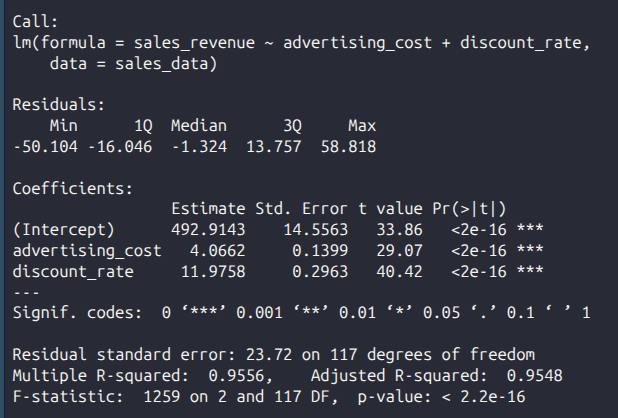
\includegraphics[width=0.92\textwidth]{./media/summary.png}
  \caption{Output \texttt{summary()} của mô hình doanh thu bán hàng. Mô hình có $R^2$ cao và các hệ số có p-value nhỏ, nhưng điều này chưa đủ để kết luận suy diễn OLS đáng tin nếu phần dư có tự tương quan.}
  \label{fig:autocorr_sales_summary}
\end{figure}

Phương trình ước lượng thu được là:
\[
  \widehat{\mathrm{sales\_revenue}}_t
  =
  492.9143
  + 4.0662\,\mathrm{advertising\_cost}_t
  + 11.9758\,\mathrm{discount\_rate}_t.
\]
Kết quả ban đầu cho thấy mô hình khớp tốt trong mẫu, nhưng cần kiểm tra phần dư theo thời gian trước khi tin vào sai số chuẩn và p-value cổ điển.

\subsubsection{Kiểm Định Durbin--Watson Trong R}

\begin{lstlisting}[style=Rstyle]
library(lmtest)

dwtest(sales_model)
\end{lstlisting}

Giả thuyết kiểm định một phía thường dùng trong ví dụ này là:
\[
  H_0:\rho=0
  \qquad \text{và} \qquad
  H_1:\rho>0.
\]

\begin{figure}[H]
  \centering
  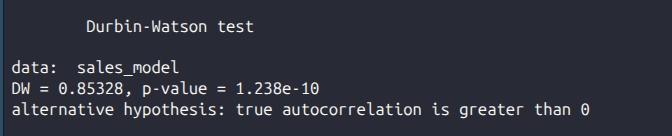
\includegraphics[width=0.82\textwidth]{./media/d.png}
  \caption{Kết quả kiểm định Durbin--Watson. p-value nhỏ và thống kê $d<2$ cho thấy bằng chứng về tự tương quan dương bậc 1.}
  \label{fig:autocorr_dw_result}
\end{figure}

\subsubsection{Kiểm Định Breusch--Godfrey Trong R}

Kiểm định tự tương quan đến bậc 1:
\begin{lstlisting}[style=Rstyle]
bgtest(sales_model, order = 1)
\end{lstlisting}

\begin{figure}[H]
  \centering
  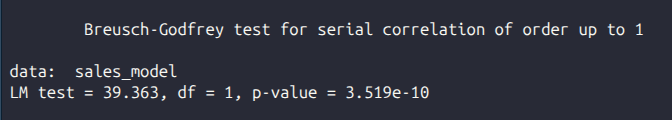
\includegraphics[width=0.82\textwidth]{./media/bg_1.png}
  \caption{Kết quả Breusch--Godfrey bậc 1. p-value nhỏ hơn $0.05$ cho thấy có bằng chứng tự tương quan bậc 1.}
  \label{fig:autocorr_bg1_result}
\end{figure}

Kiểm định tự tương quan đến bậc 2:
\begin{lstlisting}[style=Rstyle]
bgtest(sales_model, order = 2)
\end{lstlisting}

\begin{figure}[H]
  \centering
  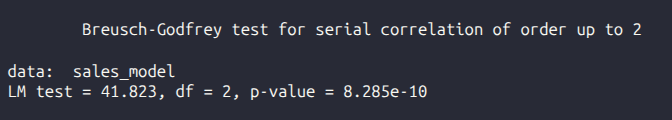
\includegraphics[width=0.82\textwidth]{./media/bg_2.png}
  \caption{Kết quả Breusch--Godfrey bậc 2. Bác bỏ $H_0$ nghĩa là có ít nhất một hệ số tự tương quan trong hai bậc đầu khác $0$.}
  \label{fig:autocorr_bg2_result}
\end{figure}

\subsubsection{Kết Luận Ví Dụ}

Cả Durbin--Watson và Breusch--Godfrey đều bác bỏ giả thuyết không có tự tương quan. Vì vậy, dù mô hình có $R^2$ cao và các biến độc lập có ý nghĩa thống kê, sai số chuẩn, p-value và các kết luận suy diễn OLS thông thường có thể không đáng tin cậy.

\begin{notebox}
\textbf{Bài học thực hành.} Với dữ liệu có thứ tự thời gian, output hồi quy chỉ là bước đầu. Cần kiểm tra phần dư theo thời gian và dùng kiểm định tự tương quan trước khi kết luận về ý nghĩa thống kê của hệ số.
\end{notebox}

% -----------------------------------------------------------------------------
